%\chapter{Multivariate Analysis}
\section{Multivariate Analysis}
\label{sec:MVA}
The difficulty of the VBS semi-leptonic channel is its low signal background ratio. 
Even after applying the event selection described in section~\ref{sec:eventselection}, they are still many backgrounds left. 
In order to improve the sensitivity of the EW VV+jj signals with respect to the other backgrounds, a machine learning approach is used for this analysis.
The idea is to use several features that have differences between signal and background and make new phase space optimized to get better separation. 
The machine learning architecture learns the features of the several input distributions and produces a single output distribution optimized to separate the signal and background.
The produced distributions in the SRs are used as a final discriminant in the final fitting to extract the signal strength.

\subsection{Architecture of the multivariate analysis}
The architecture used for this analysis is a Recurrent Neural Network (RNN) - based DeepLearning technique.
RNN~\cite{Sherstinsky_2020} is a class of the neural network architecture, recently used for the flavor tagging~\cite{ATL-PHYS-PUB-2017-003} or VV semi-leptonic resonant search~\cite{HDBS-2018-10} that has the similar final states with diboson with extra jets in ATLAS experiment.
One of the general features of the RNN is using the output in each layer recurrently; unlike conventional deep learning techniques, the output of the middle layers is used as an input hence it learns the relation of the previous sequence input as visualized in figure~\ref{fig:RNNmodel}. 
\begin{figure}[H]
    \centering
    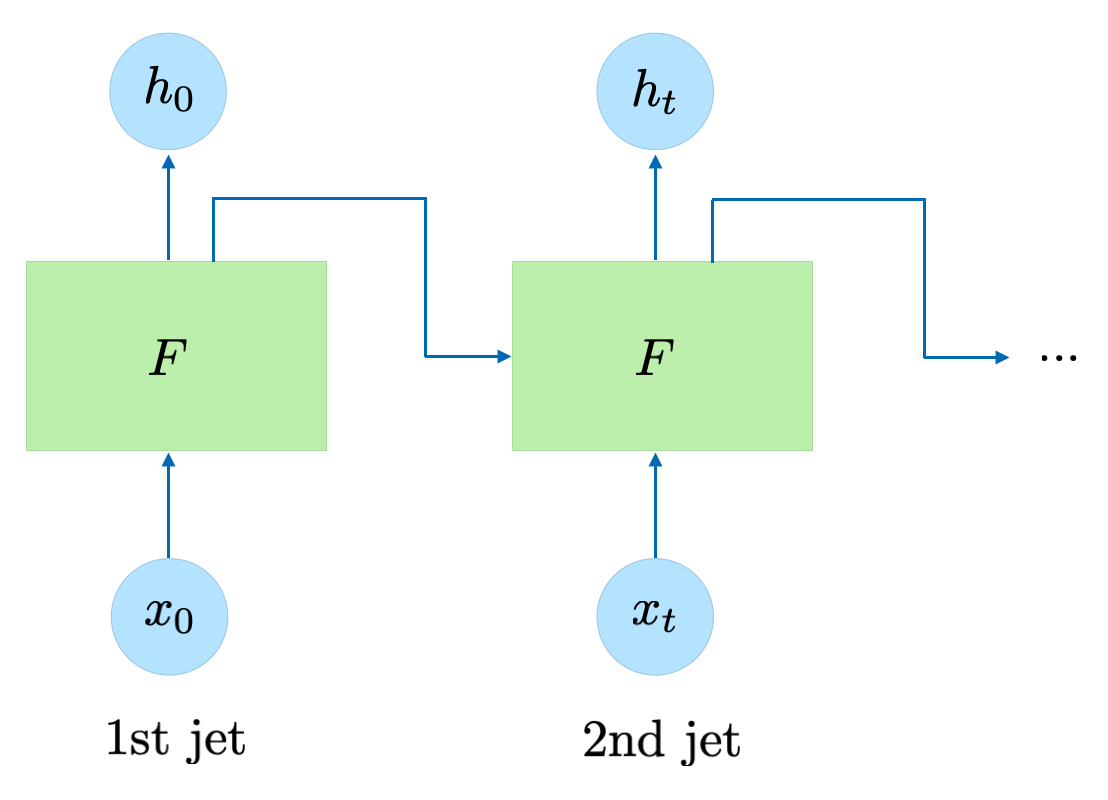
\includegraphics[width=0.6\textwidth]{figures/RNNmodel}
    \caption{The simple visualization of the RNN. $x$ is an input layer and $F$ is an intermediate layer, and $h$ is an output layer. The inputs are used recurrently by repeating the process of assigning the result of an operation performed in the intermediate layer to itself (intermediate layer) again for the next jet.
    }
    \label{fig:RNNmodel}
\end{figure}
The virtue of using RNN in this analysis is we do not need to fix the number of inputs when using it.
The jet multiplicity can be used with RNN since it is a variable feature event by event and cannot be fixed as the input value.
%, the RNN can handle this kind of input sequence naturally.
The RNN is built with the Keras~\cite{chollet2015keras}. 
Tensorflow package~\cite{tensorflow2015-whitepaper} is used as a backend for mathematical computation. 
The RNN has 2 hidden layers with 25 recurrent cells to exploit the hidden correlation of the input sequence.
Further details on the technical setups are summarized in Appendix~\ref{app:RNNsetup}.

\subsection{Input variables and setups}
The $p_\mathrm{T}, \eta, \phi, E$, of the small-R jets as well as the track multiplicity ($n_{Tracks}$) are used as inputs in a recurrent way. 
As actual input information, only these low-level information of $p_\mathrm{T}$ ordered small-R jets are used regardless they are signal and forward jets or other jets. 
The maximum variable length given by the jets multiplicity, is fixed to be 5 in this analysis. 
The values are filled with a masking value if the jet is not reconstructed in the event, and the tool knows to consider only the actual jets during the training phase according to the Keras RNN implementation. 
The maximum length (i.e. jet multiplicity) is fixed to get the significance to some extent and a rather small modeling uncertainty because of the poor modeling of the higher jet multiplicity.
%The input variables are the distributions of 4-momentum and $n_{Tracks}$ passed all event selections, which is shown in Figure... \textcolor{blue}{put input plots here}
The RNN model is trained to separate the signal from the background in each SR of each lepton channel separately, due to the different background compositions. 
In merged SR, large-R jet candidate information ($p_T, \eta, \phi, E$) is additionally used to further enhance the separation.
The output scores (RNN score) as a result of training are not used as a categorization variable by applying cut on it but used as a final discriminant for the final fitting in SRs. 
%The simple visualization of the training is shown in Figure~\ref{fig:simplenode}.
%\begin{figure}[H]
%    \centering
%    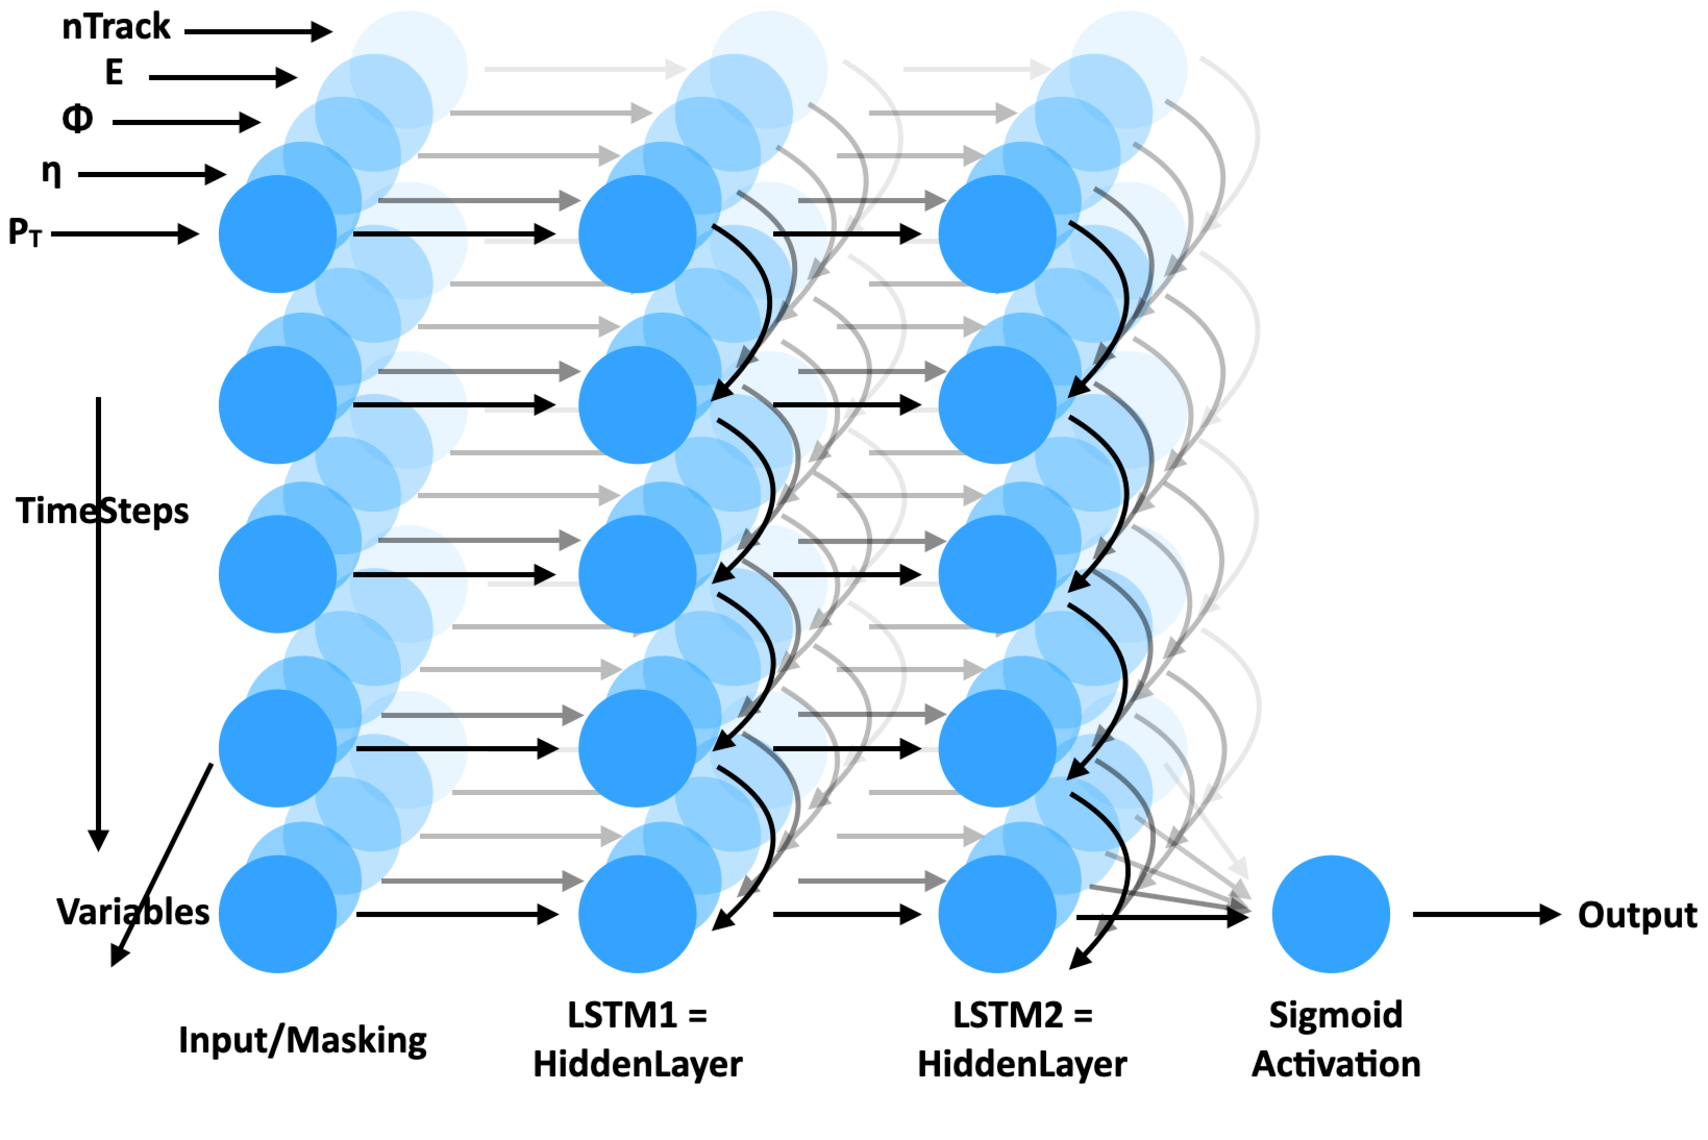
\includegraphics[width=0.7\textwidth]{figures/simplenode}
%    \caption{The visualization of the training in resolved region. 5 input variables sequences are shown and up to 5~jets.
%    }
%    \label{fig:simplenode}
%\end{figure}
%It is added and used in the combined RNN-DNN network, which is able to exploit the correlation across the tagging jets and the signal jets topology.
%The extra large-R information used as inputs are shown in Figure... \textcolor{blue}{put input plots here}
%The output RNN score in 2-lepton channel in each SRs are shown in Figure... \textcolor{blue}{put output plots here}

\subsection{Optimization of the binning}
The optimization of the binning is needed to get the optimal performance of the RNN, in order to get better significance. 
The transformation of the RNN output \cite{ATL-PHYS-PUB-2019-009} is implemented to optimize the number of bins and get the best sensitivity.
The binning of the RNN score starts from 100~bins and is summed up from the right side of the distribution until getting the best sensitivity. 
MC statistical uncertainty in each bin is required to be $<$ 20~\% to minimize the bias on fitted $\mu$~\cite{ATL-PHYS-PUB-2019-009}. 
For the current analysis, binning is required to have 15 bins.